\section{Anhang}

\subsection{Detaillierte Zeitplanung}

\begin{longtblr}[
    caption = {Detaillierte Zeitplanung},
    entry = {Detaillierte Zeitplanung},
    label = {appendix:tab:zeitplanungFein}
  ]{
    colspec = {X[1]rrr},
    width = 0.95\textwidth,
    rows = {rowsep=1.5pt},
    font = \normalsize
  }
  \textbf{Analyse}                              &               &                 & \textbf{\SI{10}{\hour}} \\
  1 Ist-Analyse                                 &               & \SI{2}{\hour}                             \\
  2 Soll-Analyse                                &               & \SI{2}{\hour}                             \\
  3 \enquote{Make or buy}-Analyse               &               & \SI{3}{\hour}                             \\
  4 Analyse der benötigten Hardware             &               & \SI{2}{\hour}                             \\
  5 Analyse des Standorts                       &               & \SI{1}{\hour}                             \\
  \textbf{Entwurf}                              &               & \rule{0pt}{4ex} & \textbf{\SI{8}{\hour}}  \\
  1 Datenbankentwurf                            &               & \SI{1}{\hour}                             \\
  2 Funktionen und Kommunikation der Services   &               & \SI{4}{\hour}                             \\
  3 Entwurf des Sensorträgers                   &               & \SI{3}{\hour}                             \\

  \textbf{Implementierung}                      &               & \rule{0pt}{4ex} & \textbf{\SI{39}{\hour}} \\
  1 Erstellung der Datenbanktabellen            &               & \SI{2}{\hour}                             \\
  2 Erstellen der RabbitMQ Exchanges            &               & \SI{1}{\hour}                             \\
  3 Erstellen des Datenspeicherservices         &               & \SI{4}{\hour}                             \\
  4 Sensorträger skizzieren und planen          &               & \SI{3}{\hour}                             \\
  5 Erstellen der Sensordaten-Abfrage-Anwendung &               & \SI{8}{\hour}                             \\
  5.1 Arduino-Logik                             & \SI{2}{\hour} &                                           \\
  5.2 Zusammenspiel Lasersensoren und Webcam    & \SI{5}{\hour} &                                           \\
  5.3 Anbindung an RabbitMQ                     & \SI{1}{\hour} &                                           \\
  6 Erstellen des Datenverarbeitungsservice     &               & \SI{18}{\hour}                            \\
  6.1 Erkennen der Versandverpackung            & \SI{8}{\hour} &                                           \\
  6.2 Auslesen des Versandlabels                & \SI{6}{\hour} &                                           \\
  6.3 Berechnung Paketgröße                     & \SI{3}{\hour} &                                           \\
  6.4 Anbindung an RabbitMQ                     & \SI{1}{\hour} &                                           \\
  7 Aufbau Sensorträger                         &               & \SI{3}{\hour}                             \\
  \textbf{Test}                                 &               & \rule{0pt}{4ex} & \textbf{\SI{5}{\hour}}  \\
  1 Code Review                                 &               & \SI{3}{\hour}                             \\
  2 Schreibtischtest                            &               & \SI{2}{\hour}                             \\

  \textbf{Einführung}                           &               & \rule{0pt}{4ex} & \textbf{\SI{6}{\hour}}  \\
  1 Inbetriebnahme der Services                 &               & \SI{4}{\hour}                             \\
  2 Abnahme durch den Teamleiter                &               & \SI{2}{\hour}                             \\

  \textbf{Dokumentation}                        &               & \rule{0pt}{4ex} & \textbf{\SI{12}{\hour}} \\
  1 Erstellung der Entwicklerdokumentation      &               & \SI{4}{\hour}                             \\
  2 Erstellung der Projektdokumentation         &               & \SI{8}{\hour}                             \\

  \hline
  \textbf{Gesamt}                               &               &                 & \textbf{\SI{80}{\hour}}
\end{longtblr}


\subsection{Ressourcenplanung}

\begin{table}[htbp]
  \centering
  \renewcommand{\arraystretch}{1.25}
  \caption{Ressourcenplanung}
  \begin{tabular}{l|l|l}
    Personal                      & Hardware                  & Software           \\
    \hline
    Auszubildender                & HP Z2 Mini G4 Workstation & Windows 10         \\
    Teammitglieder                & Server                    & Visual Studio 2022 \\
    Teamleiter \& Projektbetreuer & Custom Desktop-PC         & Visual Studio Code \\
    Product Owner                 & Arduino Mega 2560         & PyCharm CE         \\
    Techniker                     &                           & Arduino IDE        \\
    Schichtleiter Versand         &                           & DBeaver            \\
                                  &                           & Docker Desktop
  \end{tabular}
  \label{appendix:tab:ressourcen}
\end{table}


\newpage
\subsection{Angebot der Elektro Löther GmbH}

\begin{figure}[htpb]
  \centering
  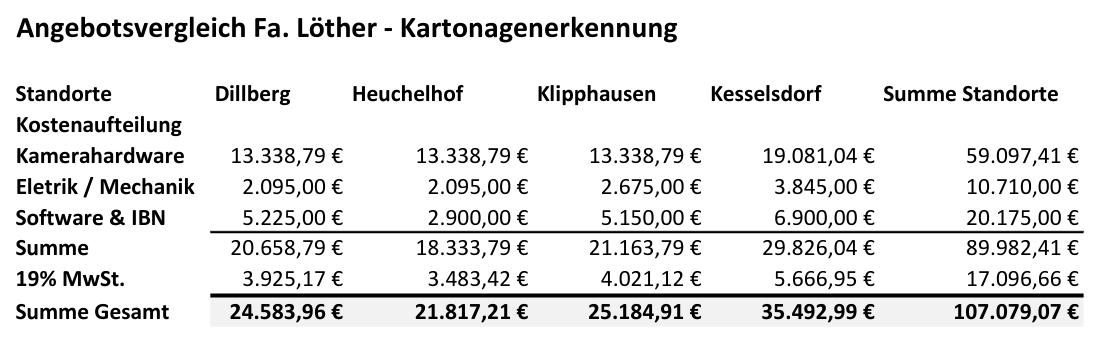
\includegraphics[width=0.9\textwidth]{./pics/AngebotLoether.png}
  \caption{Angebotsvergleich Fa. Löther -- Kartonagenerkennung}
  \label{appendix:fig:fa_loether_angebot}
\end{figure}


\subsection{Auswertung IR-Sensor}

\begin{figure}[htpb]
  \centering
  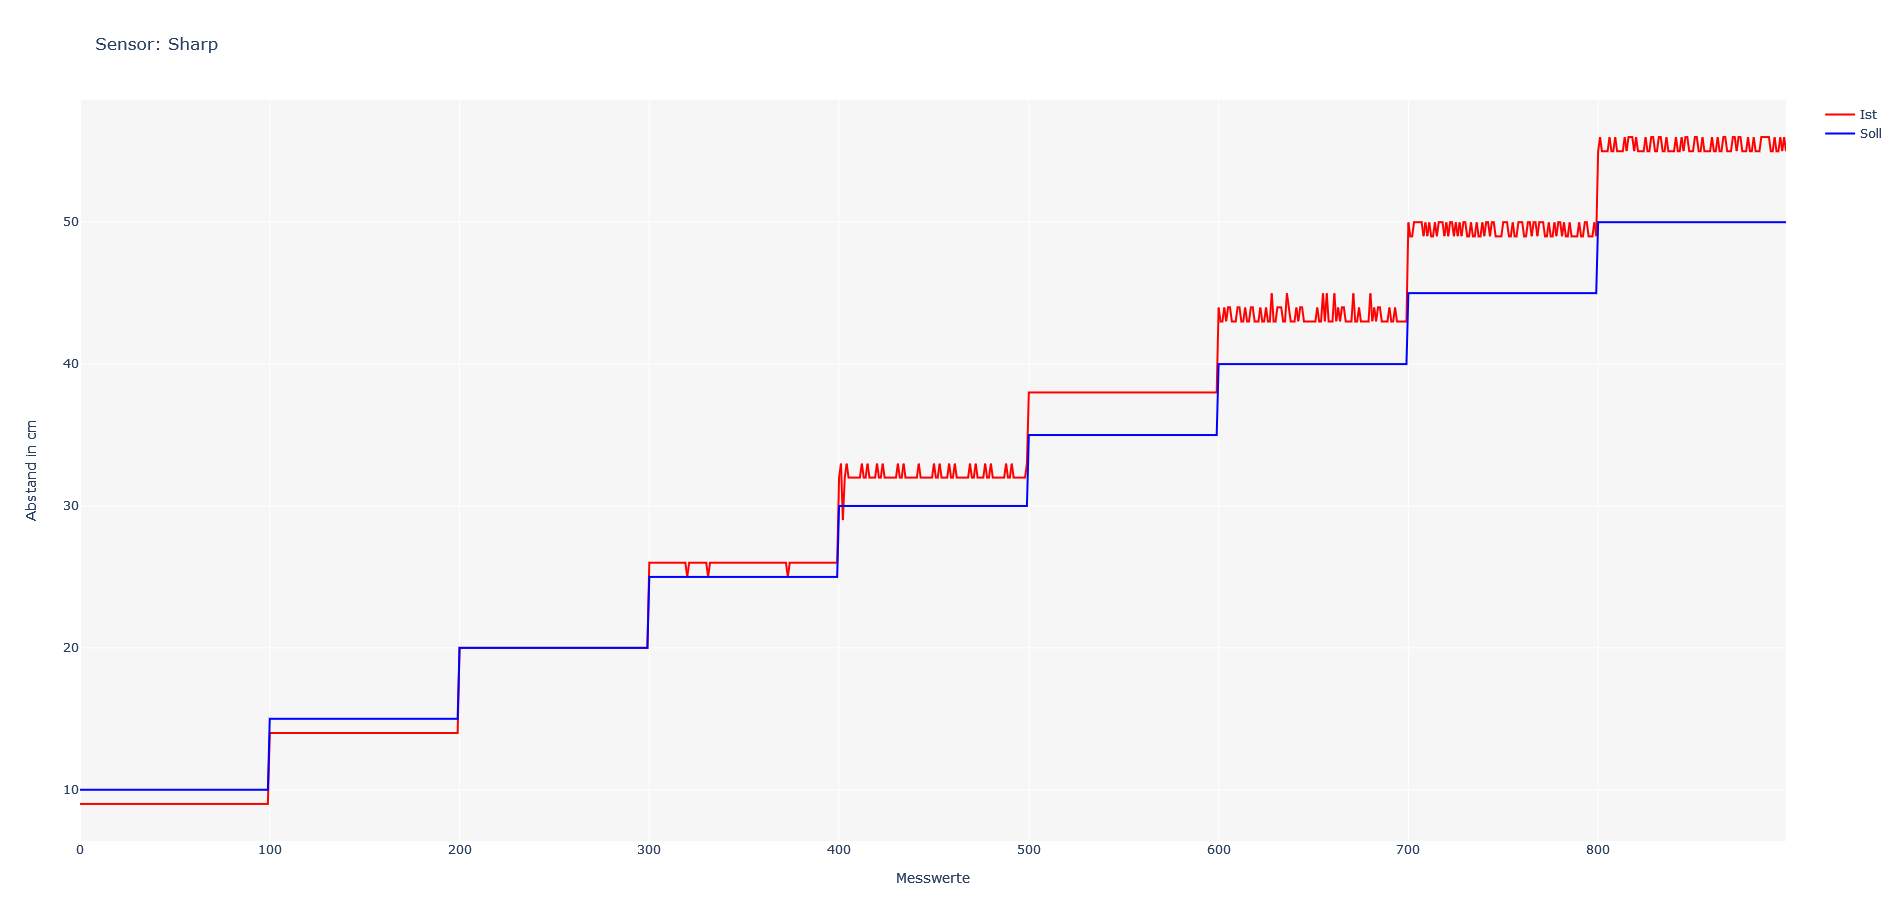
\includegraphics[width=0.95\textwidth]{./pics/plots/sharp_plot.png}
  \caption{Auswertung \ac{IR}-Sensor}
  \label{appendix:fig:irSensorAuswertung}
\end{figure}


\newpage
\subsection{Auswertung Ultraschallsensor}

\begin{figure}[htpb]
  \centering1
  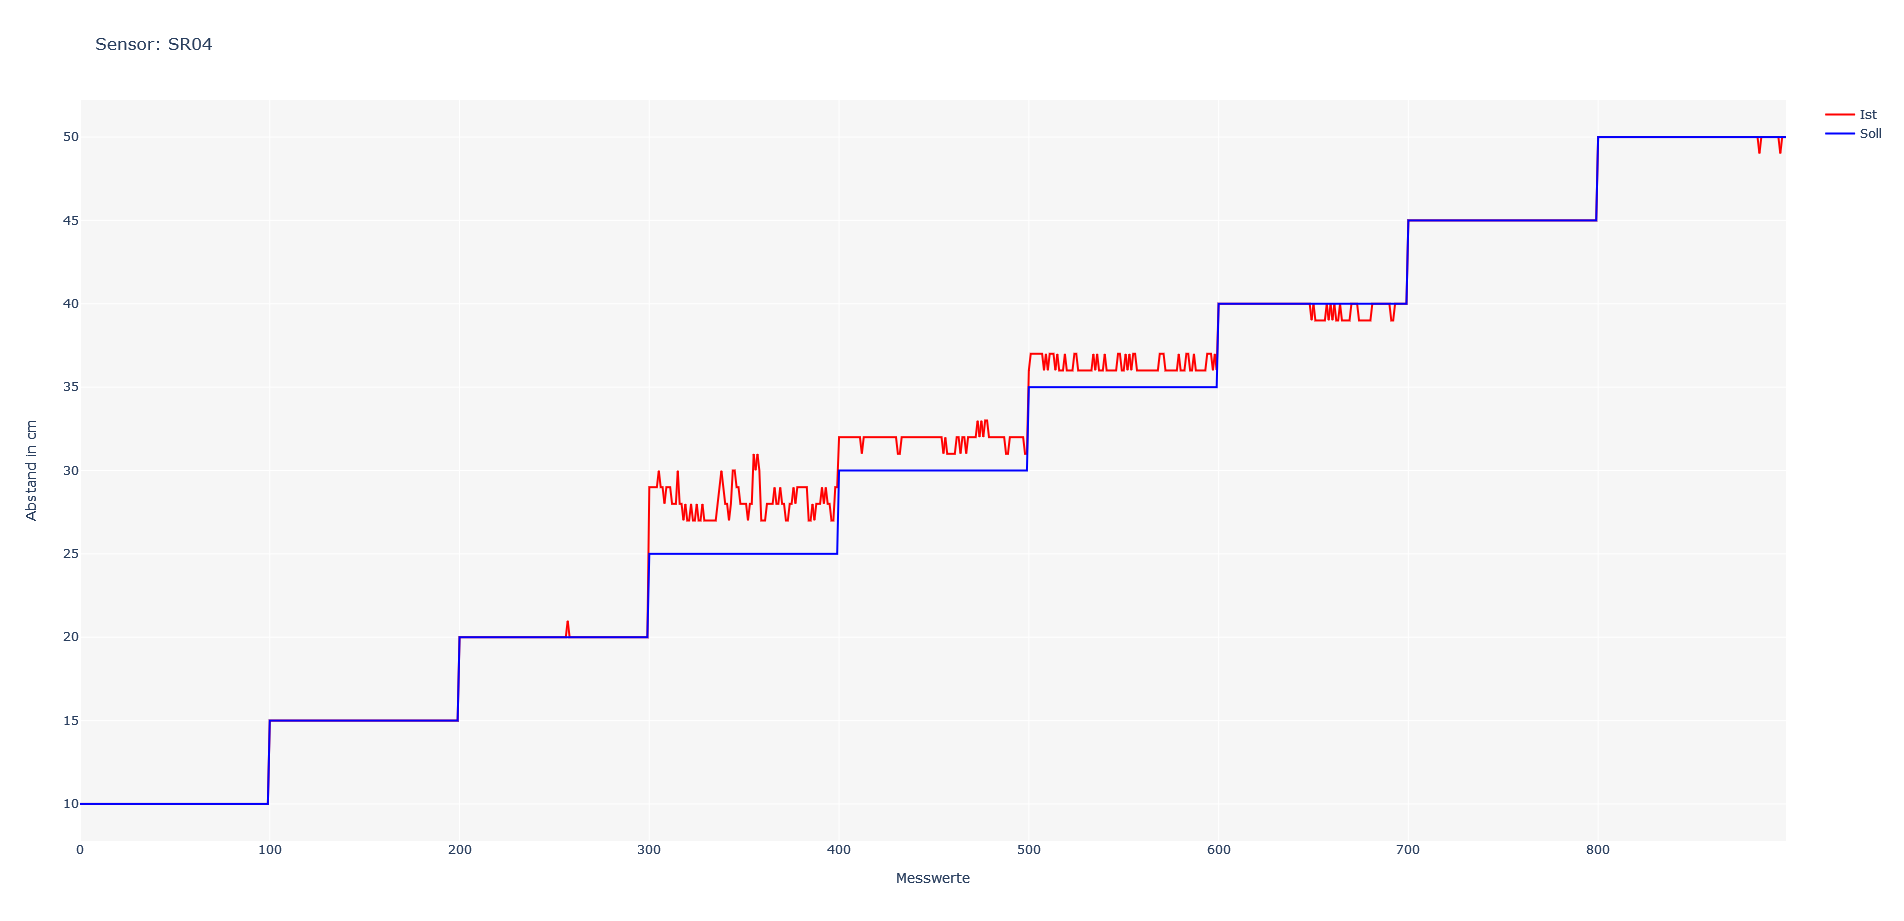
\includegraphics[width=0.95\textwidth]{./pics/plots/sr04_plot.png}
  \caption{Auswertung Ultraschallsensor}
  \label{appendix:fig:ultraSensorAuswertung}
\end{figure}


\subsection{Auswertung Lasersensor}

\begin{figure}[htpb]
  \centering
  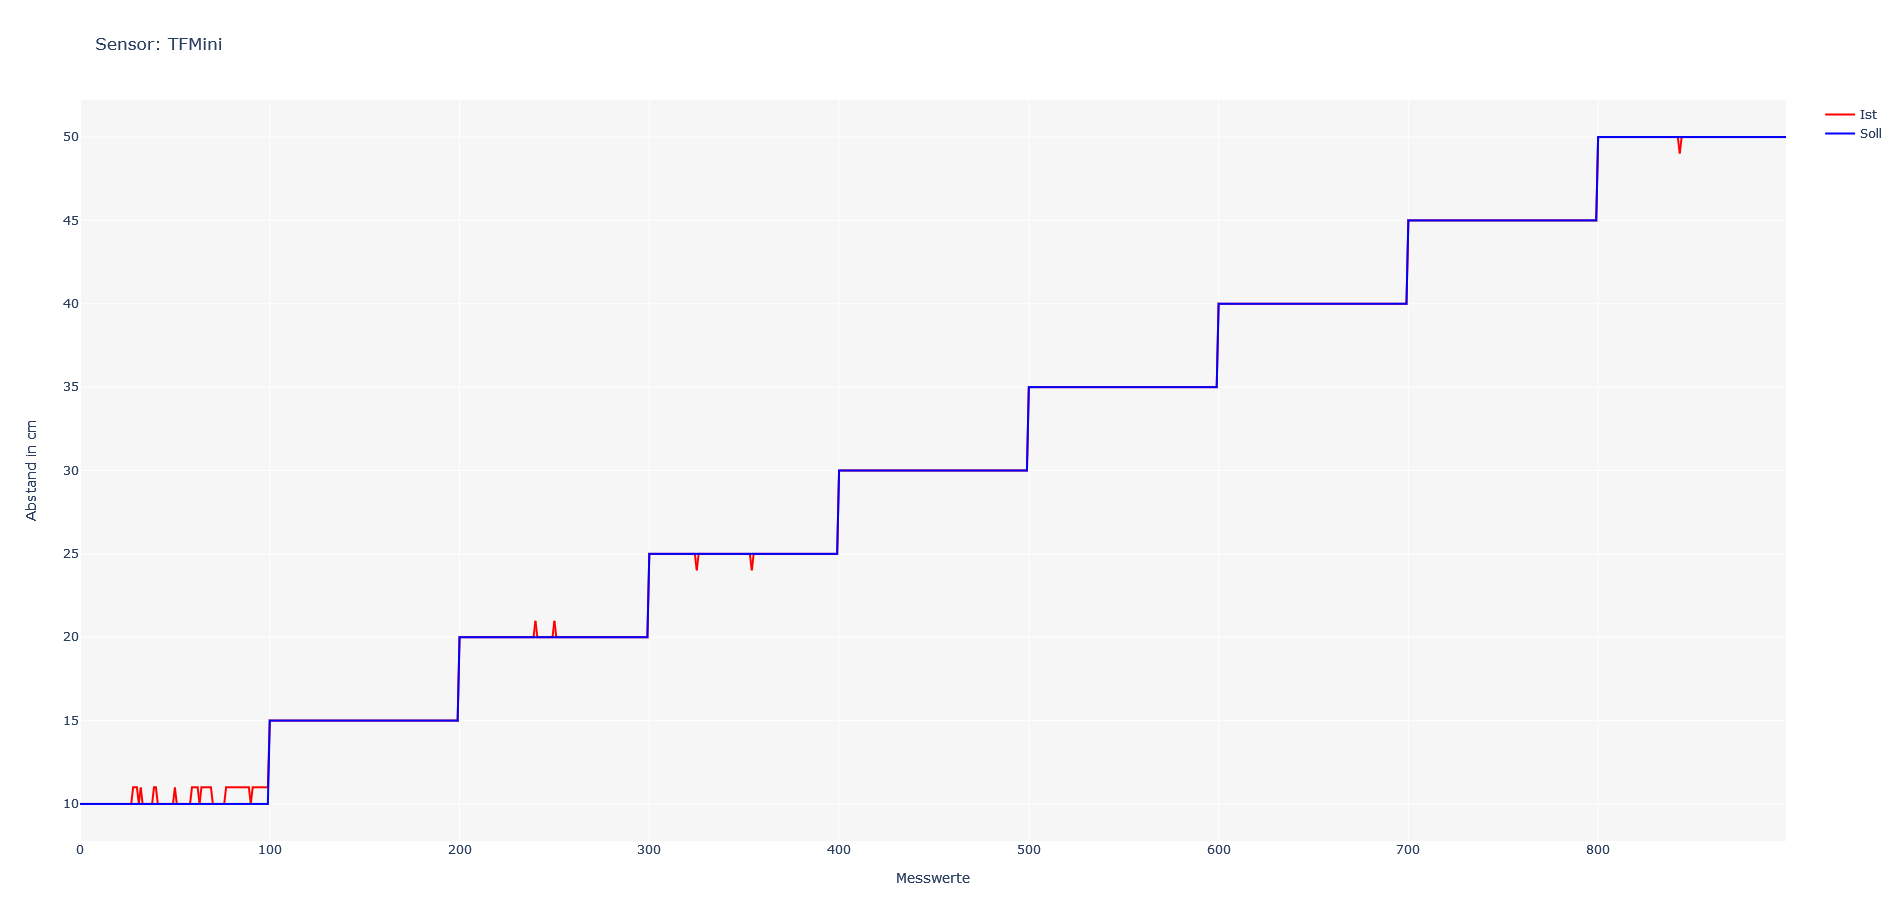
\includegraphics[width=0.95\textwidth]{./pics/plots/tfmini_plot.png}
  \caption{Auswertung Lasersensor}
  \label{appendix:fig:laserSensorAuswertung}
\end{figure}


\newpage
\subsection{Epic}

\begin{figure}[htpb]
  \centering1
  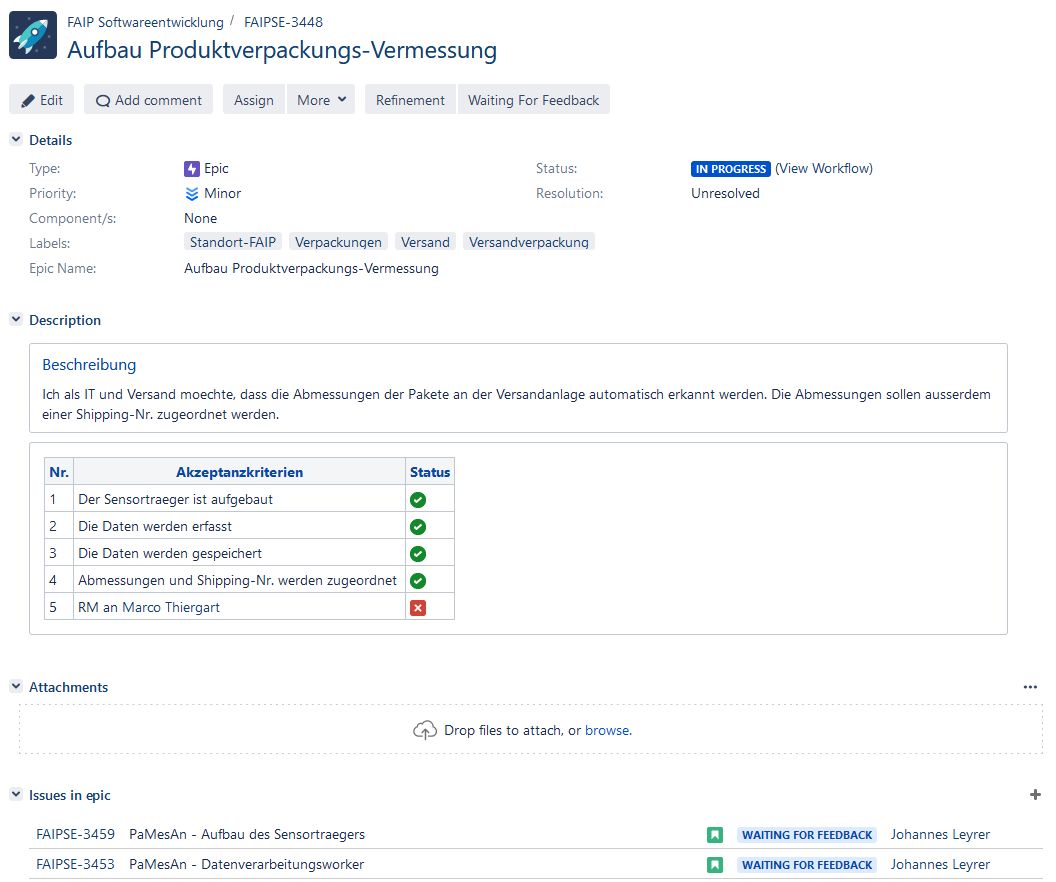
\includegraphics[width=0.95\textwidth]{./pics/Ticket.png}
  \caption{Beispiel Epic}
  \label{appendix:fig:ticket}
\end{figure}


\newpage
\subsection{Architekturdesign}

\begin{figure}[htpb]
  \centering
  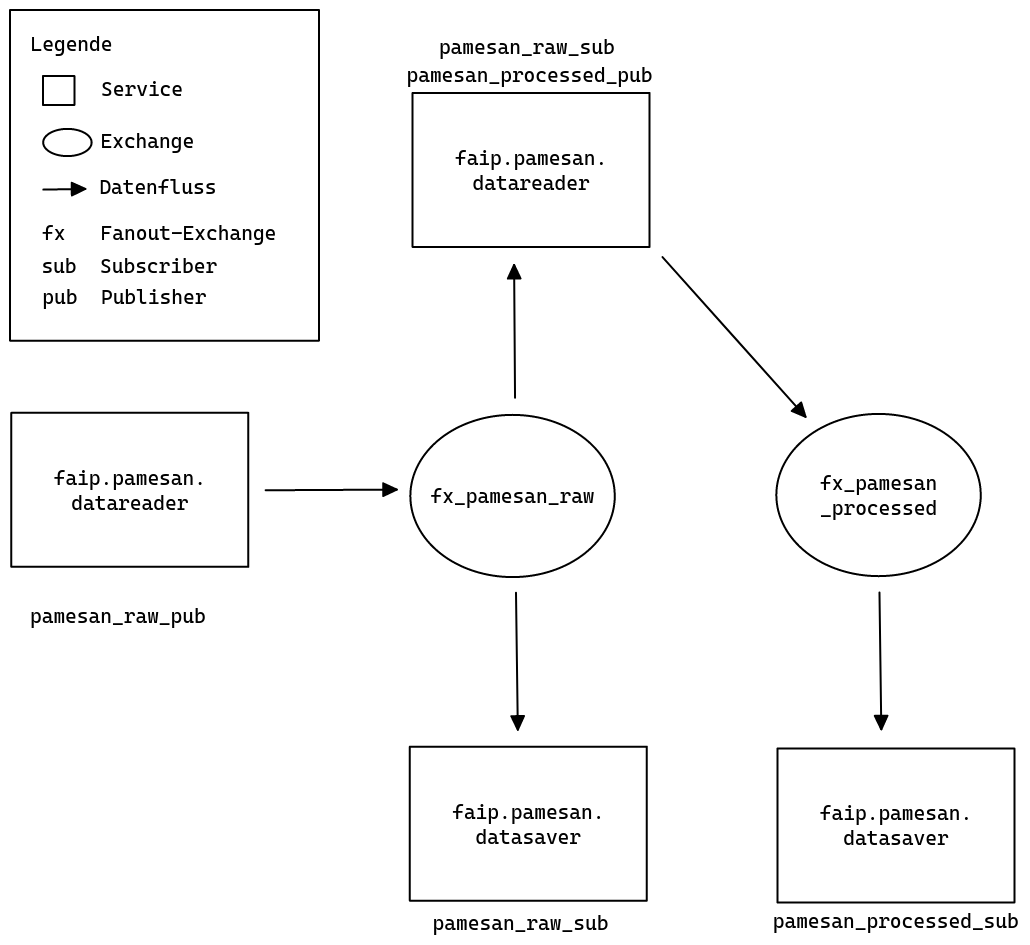
\includegraphics[width=0.85\textwidth]{./pics/Architektur.png}
  \caption{Skizze des Architekturdesigns}
  \label{appendix:fig:datenFlussDiagramm}
\end{figure}


\newpage
\subsection{Tabellenmodell}

\begin{figure}[htpb]
  \centering
  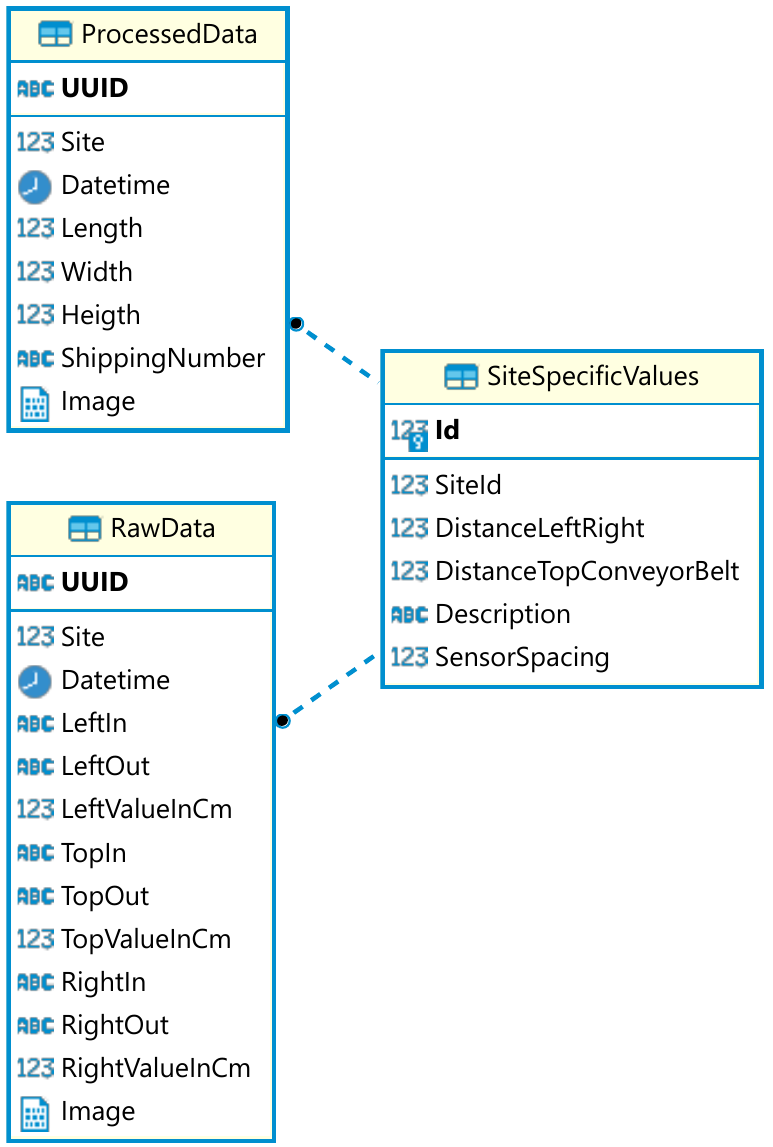
\includegraphics[width=0.65\textwidth]{./pics/Tabellenmodell.png}
  \caption{Tabellenmodell}
  \label{appendix:fig:erm}
\end{figure}


\newpage
\subsection{Skizze der Versandanlage}

\begin{figure}[htpb]
  \centering
  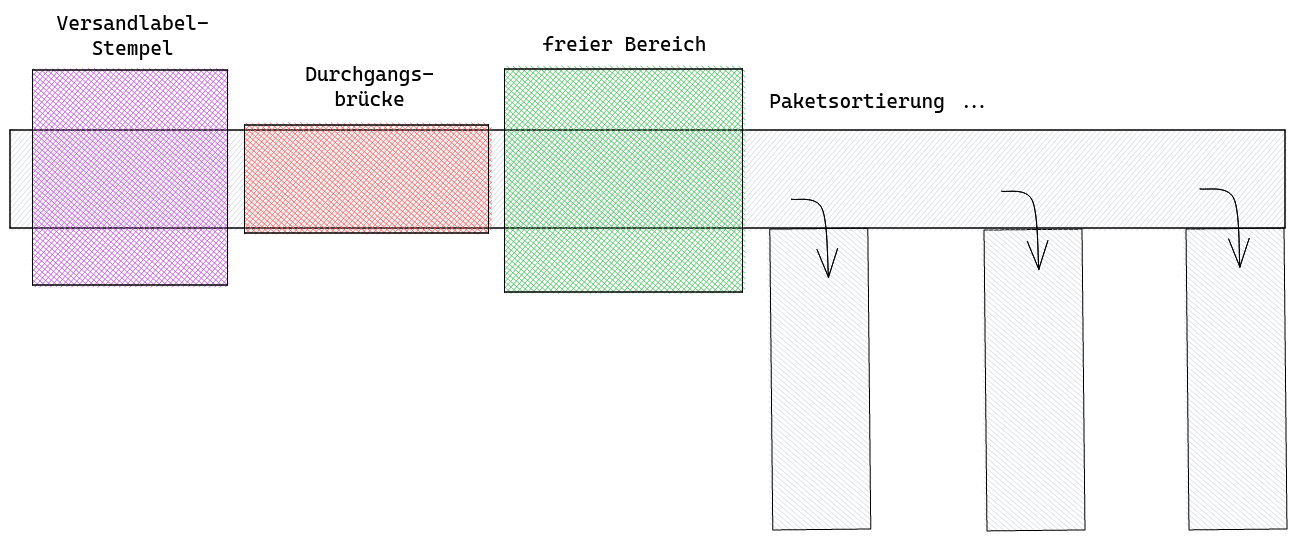
\includegraphics[angle=90,origin=c,width=0.46\textwidth]{./pics/Versandanlage.png}
  \caption{Skizze der Versandanlage}
  \label{appendix:fig:skizzeVersand}
\end{figure}


\newpage
\subsection{Sensorhalterung}

\begin{figure}[htpb]
  \centering
  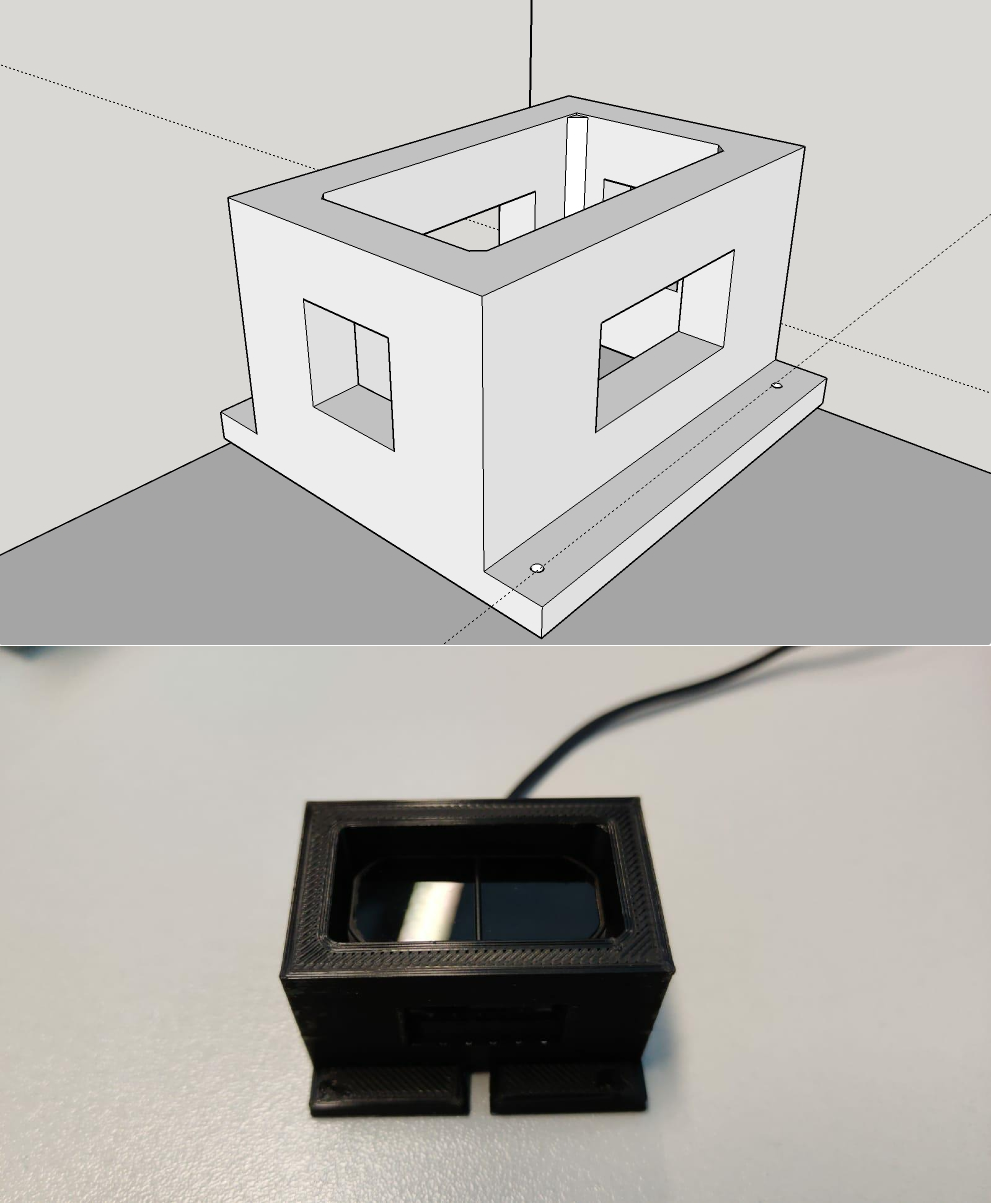
\includegraphics[width=0.85\textwidth]{./pics/thingiverse_3D.png}
  \caption{Sensorhalterung: Vorlage \autocite{thingiverse} und zusammengesetztes Endprodukt}
  \label{appendix:fig:thingiverse}
\end{figure}


\newpage
\subsection{2D-Modell des Sensorträgers}

\begin{figure}[htpb]
  \centering
  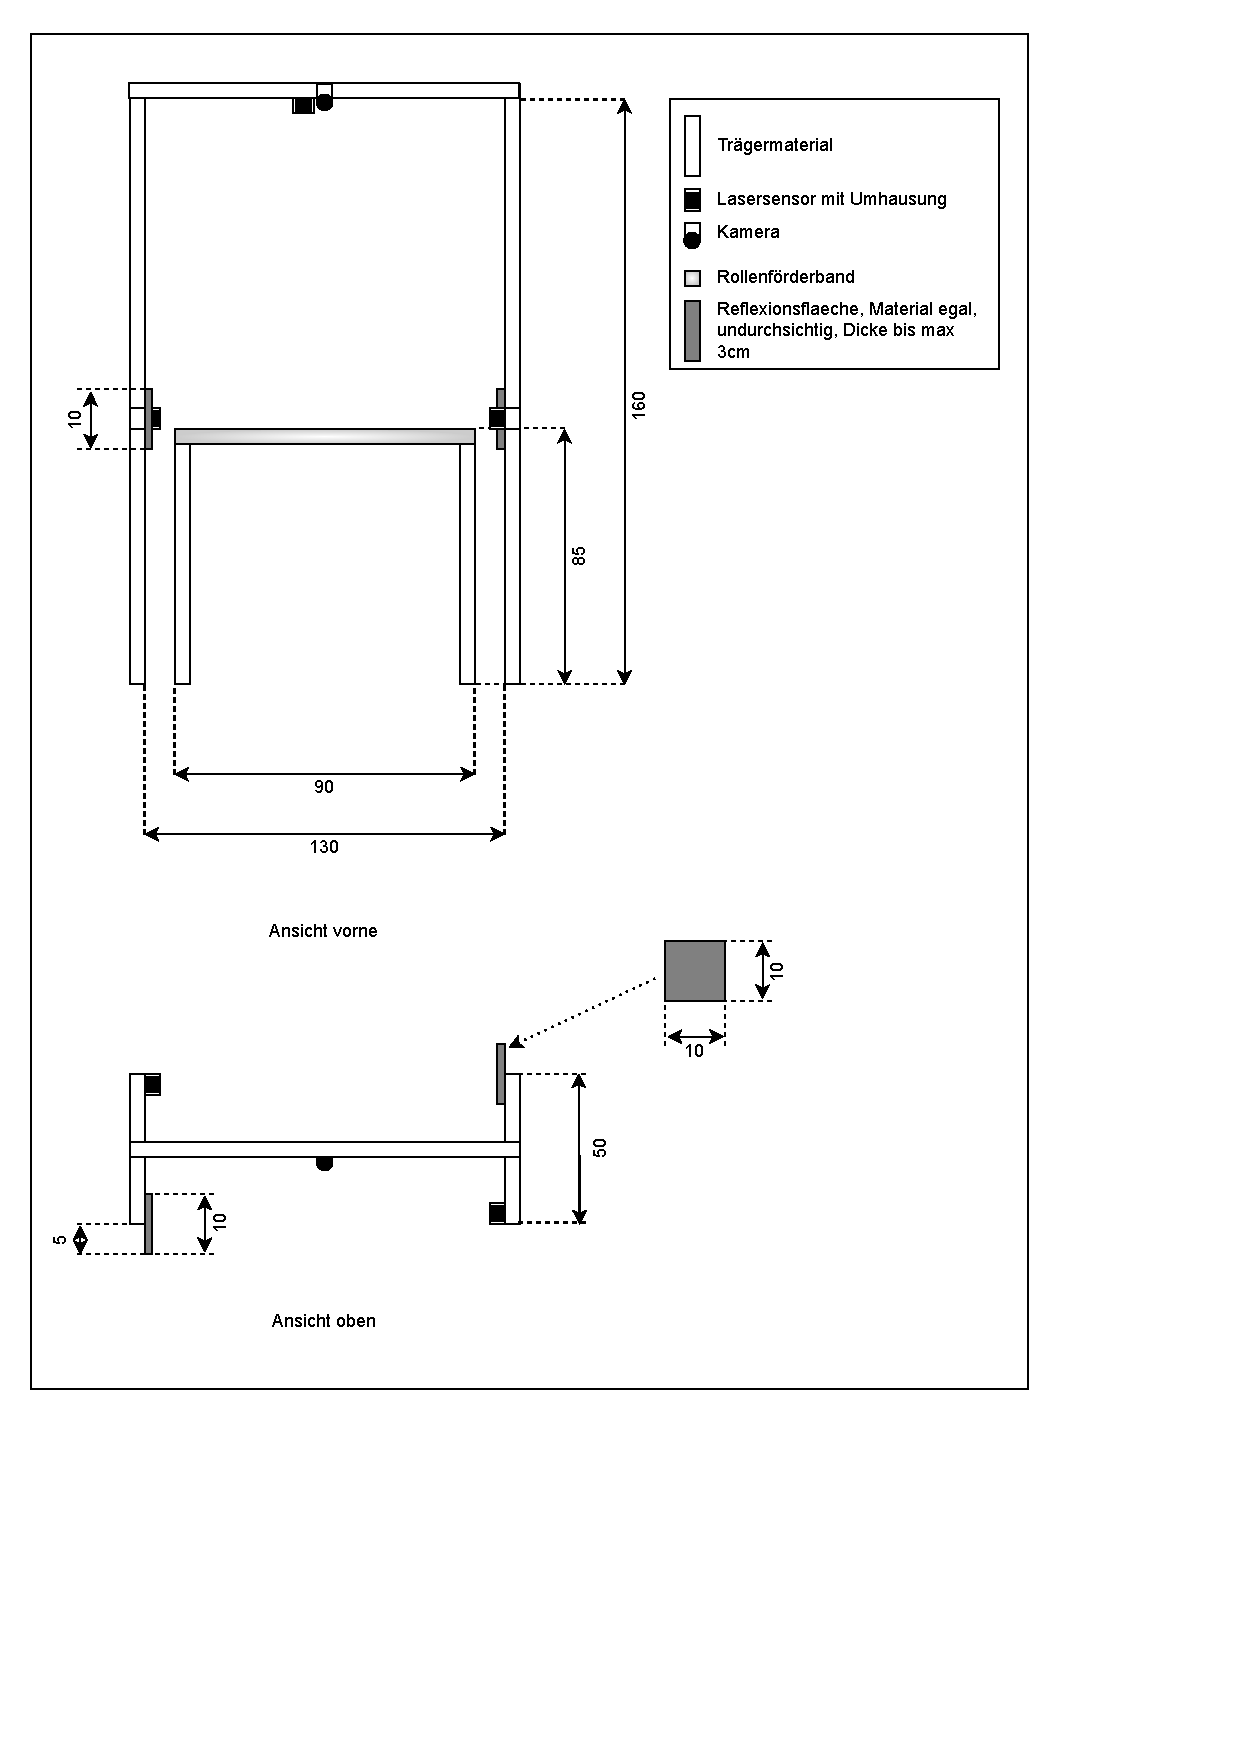
\includegraphics[trim={0 6cm 0 0}, clip, width=0.95\textwidth]{./files/Sensortraeger/Skizze_Sensor_Traeger.pdf}
  \caption{2D-Modell des Sensorträger}
  \label{appendix:pdf:sensor_traeger_skizze}
\end{figure}


\newpage
\subsection{3D-Modell des Sensorträgers}

\begin{figure}[htpb]
  \centering
  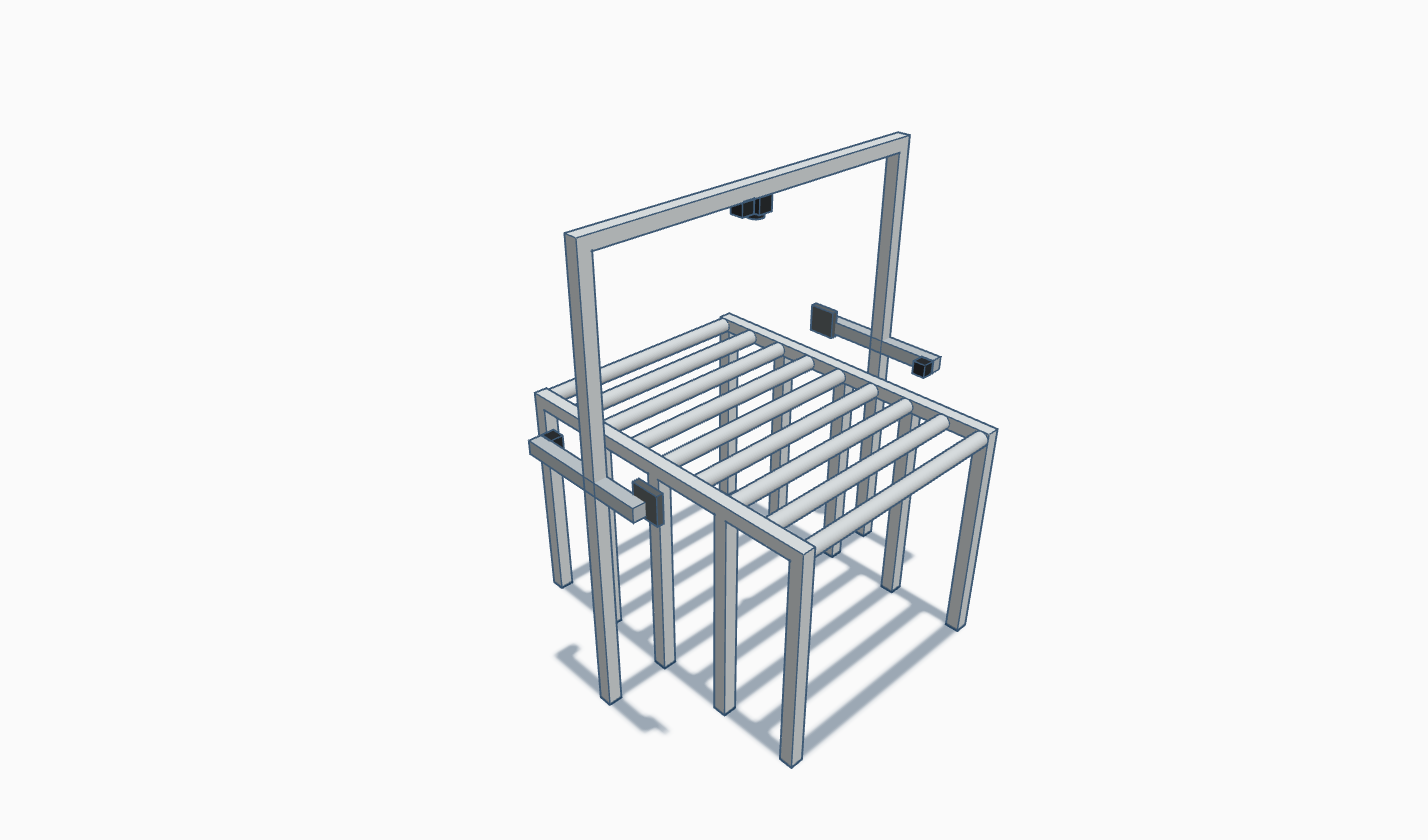
\includegraphics[trim={8cm 0 8cm 0}, clip, width=0.95\textwidth]{./files/Sensortraeger/Skizze_Sensor_Traeger_3D_verdreht.png}
  \caption{3D-Modell des Sensorträgers}
  \label{appendix:fig:sensor_traeger_3d}
\end{figure}


\newpage
\subsection{Fertiger Sensorträger}

\begin{figure}[h!]
  \centering
  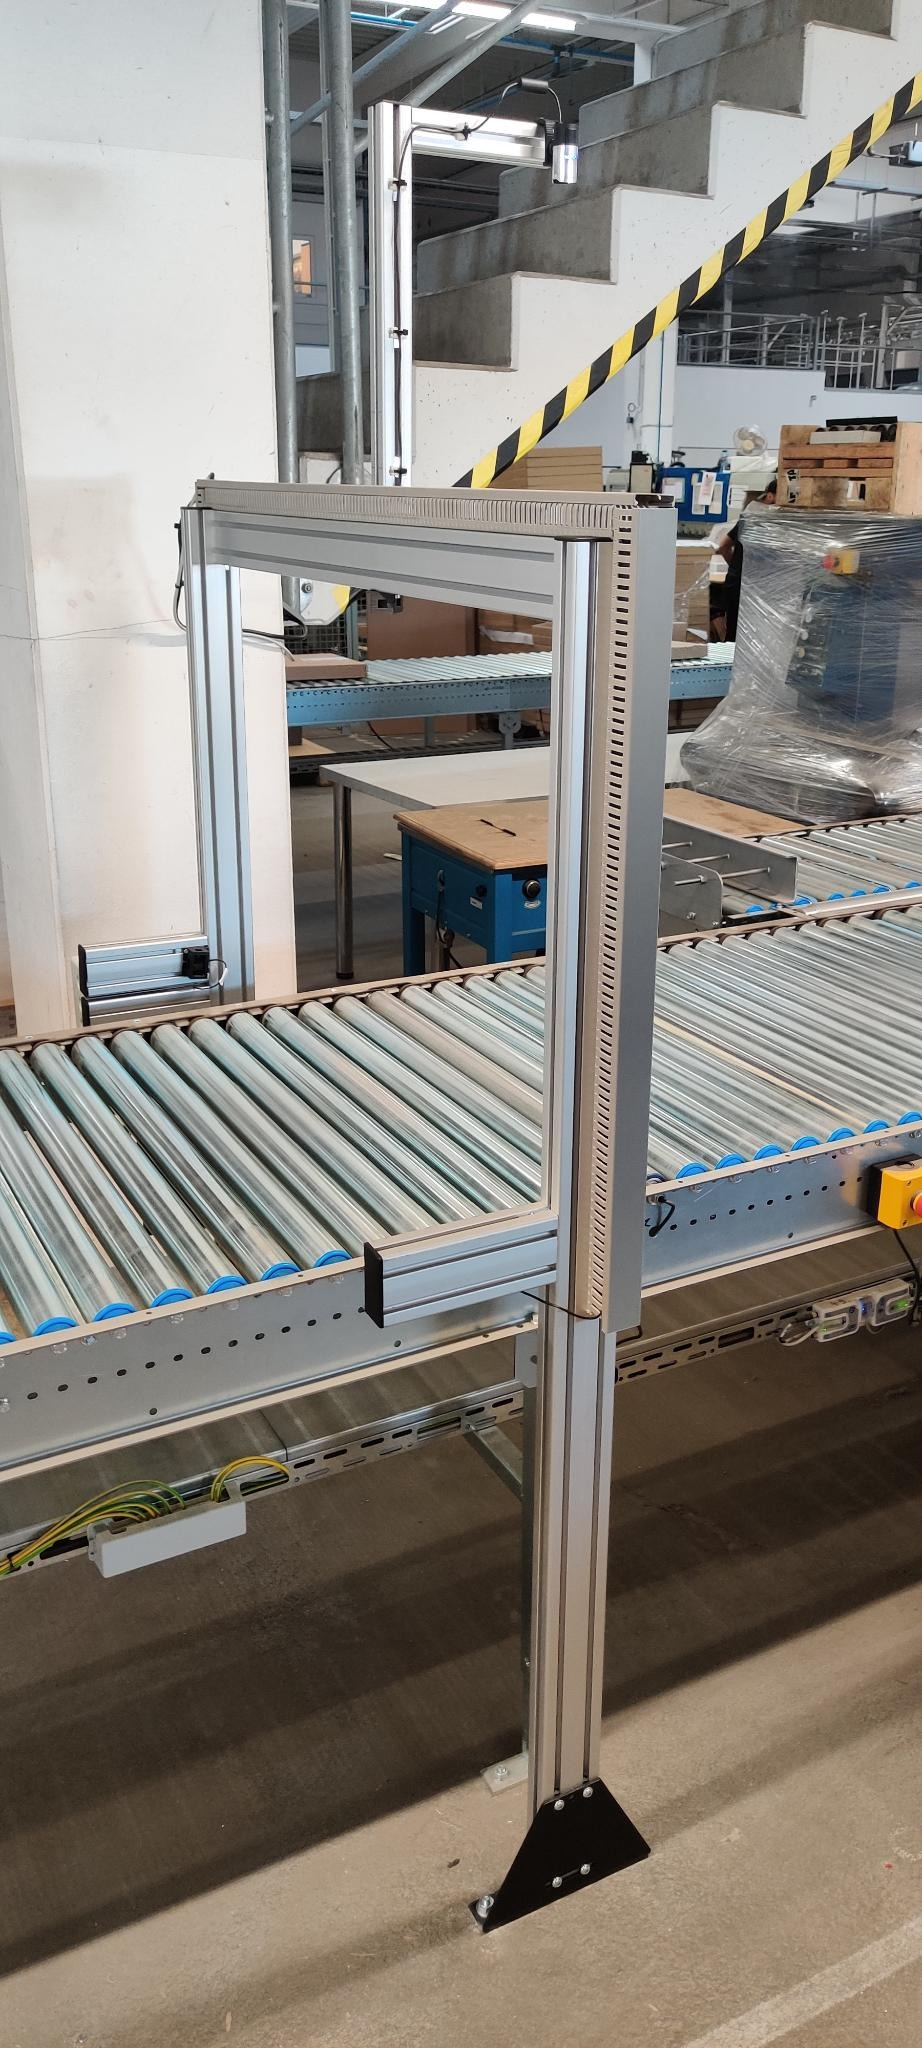
\includegraphics[width=0.55\textwidth]{./pics/Sensortraeger.jpeg}
  \caption{Fertig montierter und aufgestellter Sensorträger}
  \label{appendix:fig:sensor_traeger_fertig}
\end{figure}


\newpage
\subsection{Arduino mit Lasersensoren}

\begin{figure}[htpb]
  \centering
  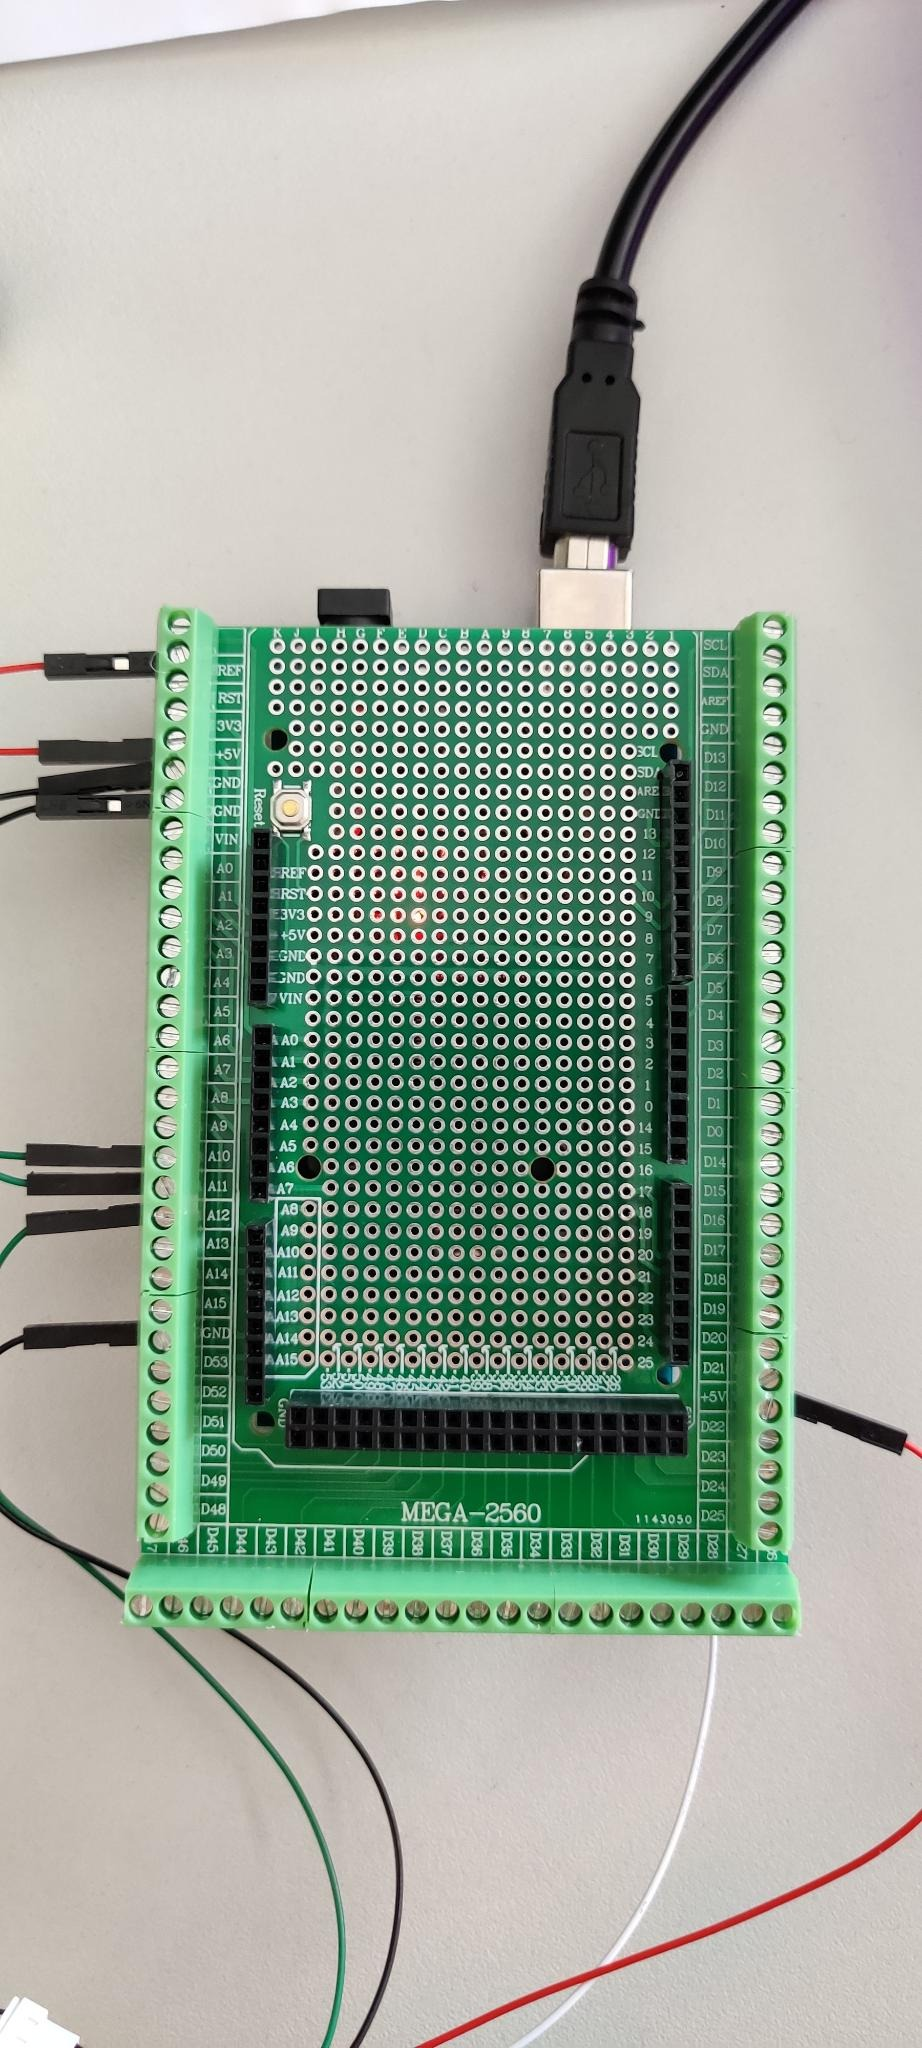
\includegraphics[width=0.45\textwidth]{./pics/Arduino.jpeg}
  \caption{Arduino mit angeschlossenen Sensoren und Shield}
  \label{appendix:fig:arduino}
\end{figure}


\newpage
\subsection{Beispiel Verwendung labelImg}

\begin{figure}[htpb]
  \centering
  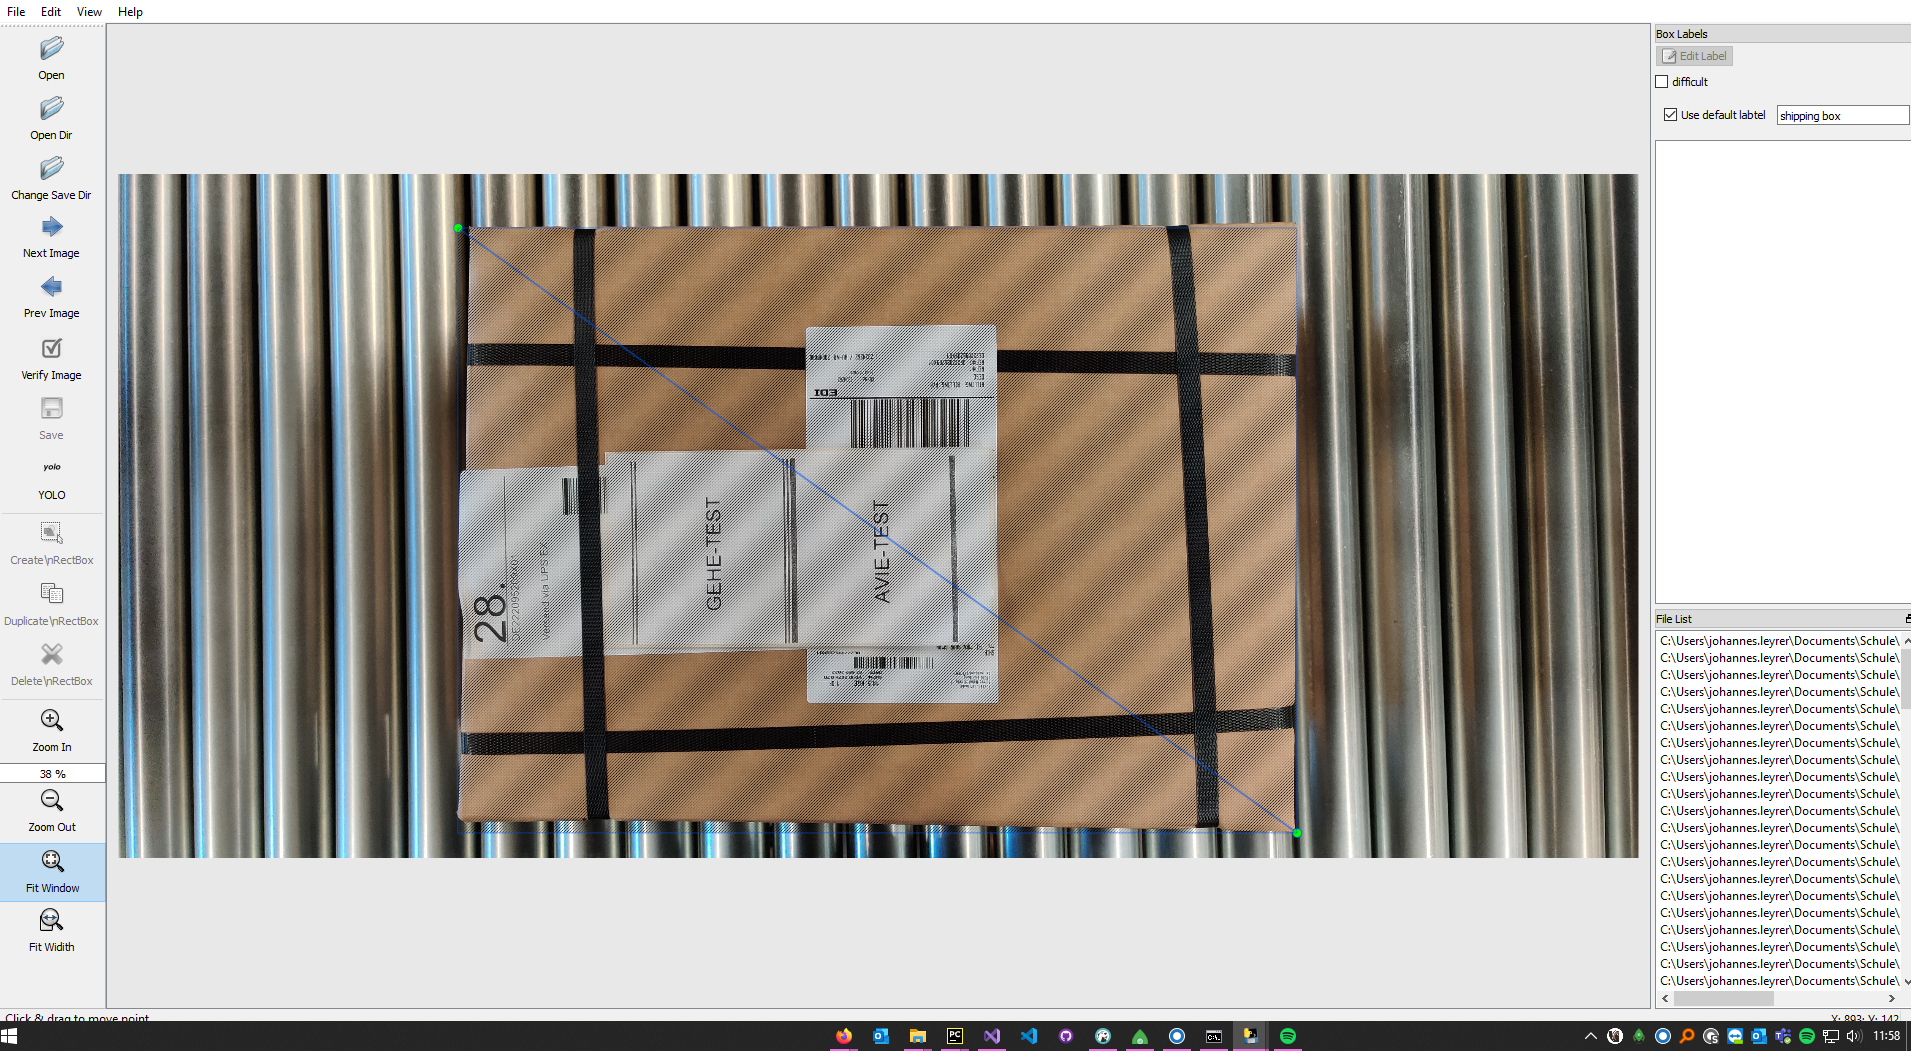
\includegraphics[width=0.95\textwidth]{./pics/labelImg.png}
  \caption{Beispiel Verwendung labelImg}
  \label{appendix:fig:labelImg}
\end{figure}


\subsection{Beispiel Barcodeerfassung}

\begin{figure}[htpb]
  \centering
  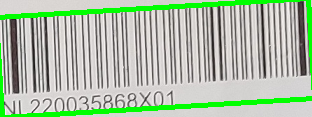
\includegraphics[width=0.75\textwidth]{./pics/barcode.png}
  \caption{Beispiel Barcodeerfassung}
  \label{appendix:fig:barcode}
\end{figure}


\newpage
\subsection{Beispiel Versandverpackungserkennung mit YOLOv7}

\begin{figure}[htpb]
  \centering
  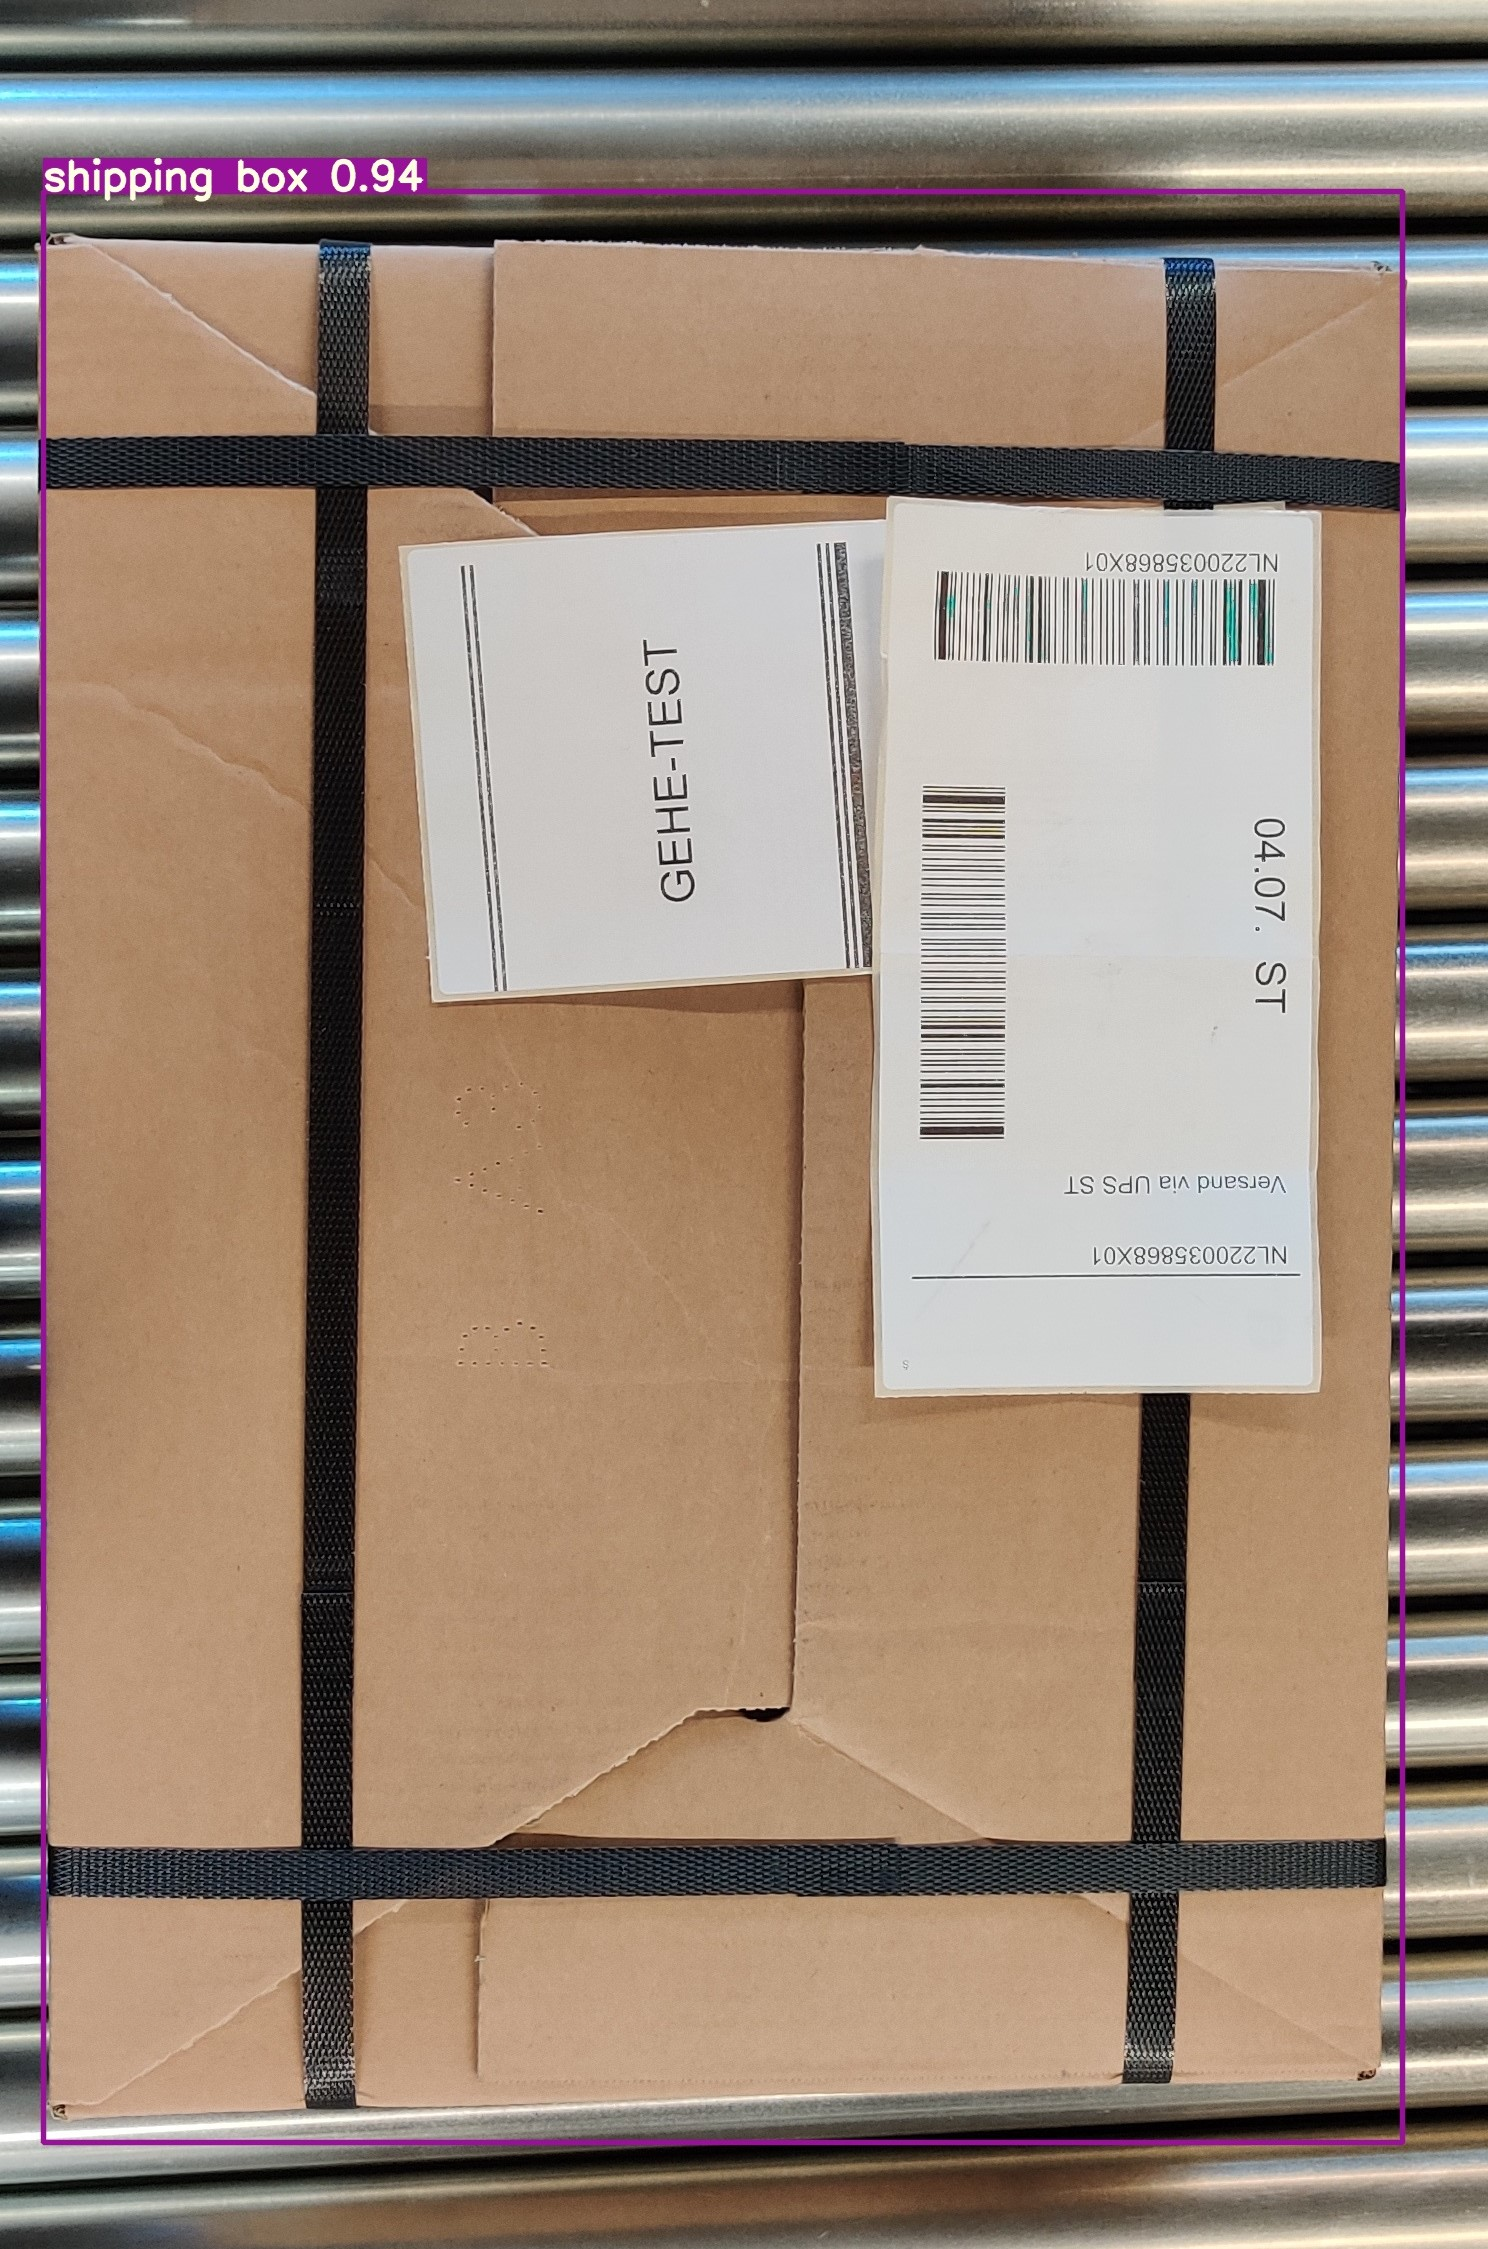
\includegraphics[width=0.65\textwidth]{./pics/detectShippingBox.jpg}
  \caption{Beispiel Versandverpackungserkennung mit Test-Label}
  \label{appendix:fig:yoloDetect}
\end{figure}


\newpage
\subsection{Beispiel Labelerfassung}

\begin{figure}[htpb]
  \centering
  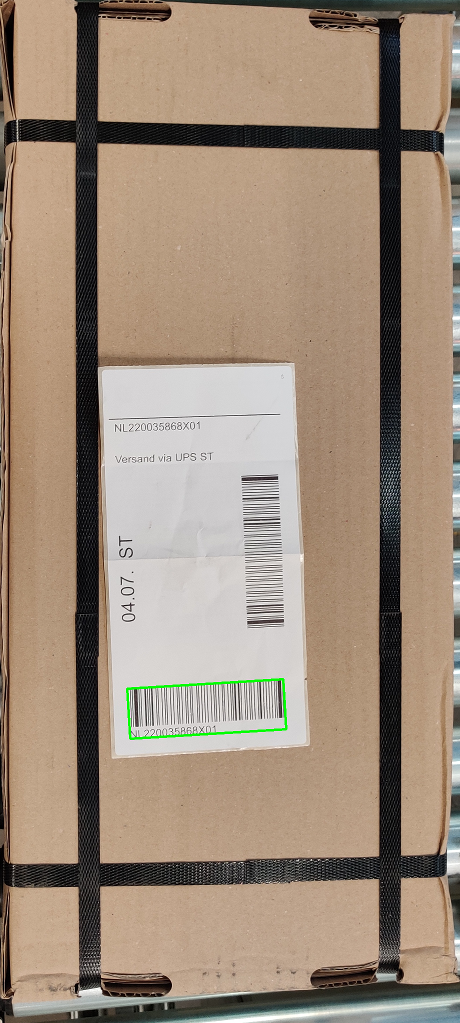
\includegraphics[width=0.45\textwidth]{./pics/foundLabel.png}
  \caption{Beispiel Erfassung des Versandlabels mit Test-Label}
  \label{appendix:fig:foundLabel}
\end{figure}


\newpage
\subsection{GitLab-CI/CD}

\begin{lstlisting}[language=gitlab-ci-cd,
    caption={.gitlab-ci.yml-Datei für \ac{CI/CD}},
    breaklines=true,
    label={appendix:lst:gitlab-ci}]
    image: docker/compose:alpine-1.29.2

    stages:
        - build
        - deploy

    before_script:
        - docker login -u $CI_DEPLOY_USER -p $CI_DEPLOY_PASSWORD
            $CI_REGISTRY

    build-prod:
        stage: build
        tags:
            - faip-swarm-prod
        script:
            - docker build -f ./FAIP.PaMesAn.DataSaver/Dockerfile -t 
                ${CI_REGISTRY_IMAGE}/prod .
            - docker push ${CI_REGISTRY_IMAGE}/prod
        only:
            refs:
                - main

    deploy-prod-raw:
        stage: deploy
        tags:
            - faip-swarm-prod
        script:
            - docker stack deploy -c prod.raw.docker-compose.yml 
                --with-registry-auth pamesan
        only:
            refs:
                - main

    deploy-prod-processed:
        stage: deploy
        tags:
            - faip-swarm-prod
        script:
            - docker stack deploy -c prod.processed.docker-compose.yml 
                --with-registry-auth pamesan
        only:
            refs:
                - main
\end{lstlisting}


\subsection{SQL-Erstellungsskript für RawData}

\begin{lstlisting}[style=sql-style,
    caption={SQL-Skript für RawData},
    breaklines=true,
    label={appendix:lst:sql_raw}]
    CREATE TABLE PAMESAN.dbo.RawData (
        UUID uniqueidentifier NOT NULL,
        Site int NOT NULL,
        [Datetime] datetime NULL,
        LeftIn nvarchar(50) COLLATE Latin1_General_CI_AS NULL,
        LeftOut nvarchar(50) COLLATE Latin1_General_CI_AS NULL,
        LeftValueInCm int NULL,
        TopIn nvarchar(50) COLLATE Latin1_General_CI_AS NULL,
        TopOut nvarchar(50) COLLATE Latin1_General_CI_AS NULL,
        TopValueInCm int NULL,
        RightIn nvarchar(50) COLLATE Latin1_General_CI_AS NULL,
        RightOut nvarchar(50) COLLATE Latin1_General_CI_AS NULL,
        RightValueInCm int NULL,
        [Image] varbinary(MAX) NULL,
        CONSTRAINT PK_RawData PRIMARY KEY (UUID),
        CONSTRAINT RawData_FK FOREIGN KEY (Site) REFERENCES PAMESAN.dbo.SiteSpecificValues(Id)
    );
\end{lstlisting}







% \subsection{Bewertung der CO\texorpdfstring{$_2$}{TEXT} Konzentration in der Raumluft nach \ac{DGUV} \ac{ASR} A3.6}

% \begin{table}[htbp]
%   \centering
%   \renewcommand{\arraystretch}{1.25}
%   \caption{Bewertung der CO$_2$ Konzentration in der Raumluft nach \ac{DGUV} \ac{ASR} A3.6 \autocite{ASR}}
%   \begin{tabular}{c|p{0.6\textwidth}}
%     CO$_2$-Konzentration in \ac{ppm} & Maßnahmen                                                                                                                  \\
%     \hline
%     $<$1000                          & $\bullet$ Keine weiteren Maßnahmen (sofern durch die Raumnutzung kein Konzentrationsanstieg über 1000 ppm zu erwarten ist) \\
%     \hline
%     1000-2000                        & $\bullet$ Lüftungsverhalten überprüfen und verbessern                                                                      \\
%                                      & $\bullet$ Lüftungsplan aufstellen (z. B. Verantwortlichkeiten festlegen)                                                   \\
%                                      & $\bullet$ Lüftungsmaßnahme (z. B. Außenluftvolumenstrom oder Luftwechsel erhöhen)                                          \\
%     \hline
%     $>$2000                          & $\bullet$ weitergehende Maßnahmen erforderlich (z. B. verstärkte Lüftung, Reduzierung der Personenzahl im Raum)            \\
%   \end{tabular}
%   \label{appendix:tab:dguv_table_co2}
% \end{table}

% \subsection{Bewertung der CO\texorpdfstring{$_2$}{TEXT} Konzentration in der Raumluft nach DIN EN 16798-1}

% \begin{table}[htbp]
%   \centering
%   \renewcommand{\arraystretch}{1.25}
%   \caption{Bewertung der CO$_2$ Konzentration in der Raumluft nach DIN EN 16798-1 \autocite{din_en_16798}}
%   \begin{tabular}{c|p{0.6\textwidth}}
%     CO$_2$-Konzentration in \ac{ppm} & Beschreibung              \\
%     \hline
%     $<$950                           & Hohe Raumluftqualität     \\
%     950-1200                         & Mittlere Raumluftqualität \\
%     1200-1750                        & Mäßige Raumluftqualität   \\
%     $>$1750                          & Niedrige Raumluftqualität \\
%   \end{tabular}
%   \label{appendix:tab:din_table_co2}
% \end{table}
